\section{Introduction}
\label{sec:introduction}

% state the learning objective 
The aim of this laboratory work regarding the topics studied in the first three weeks of the course was to analyse a circuit constituted of an independent voltage source, an independent voltage source, a voltage controlled dependent current source, a current controlled dependent voltage source and seven resistors, as shown in the Figure~\ref{fig:t1draw} below.
. For this, a theorical analysis was made using both node and mesh methods, whose results will be discussed in section one. To validate these results, a simulation was conducted, as will apeear in section 2.


The forementioned analysis was divided into a theoretical one, presented in section ~\ref{sec:analysis}.In order to be able to validate the results obtained, a simulation was also conducted, as shown in Section ~\ref{sec:simulation}. The results were then compared (Section~\ref{sec:simulation}), and the conclusions of the group summarized in Section~\ref{sec:conclusion}.


\begin{figure}[h] \centering
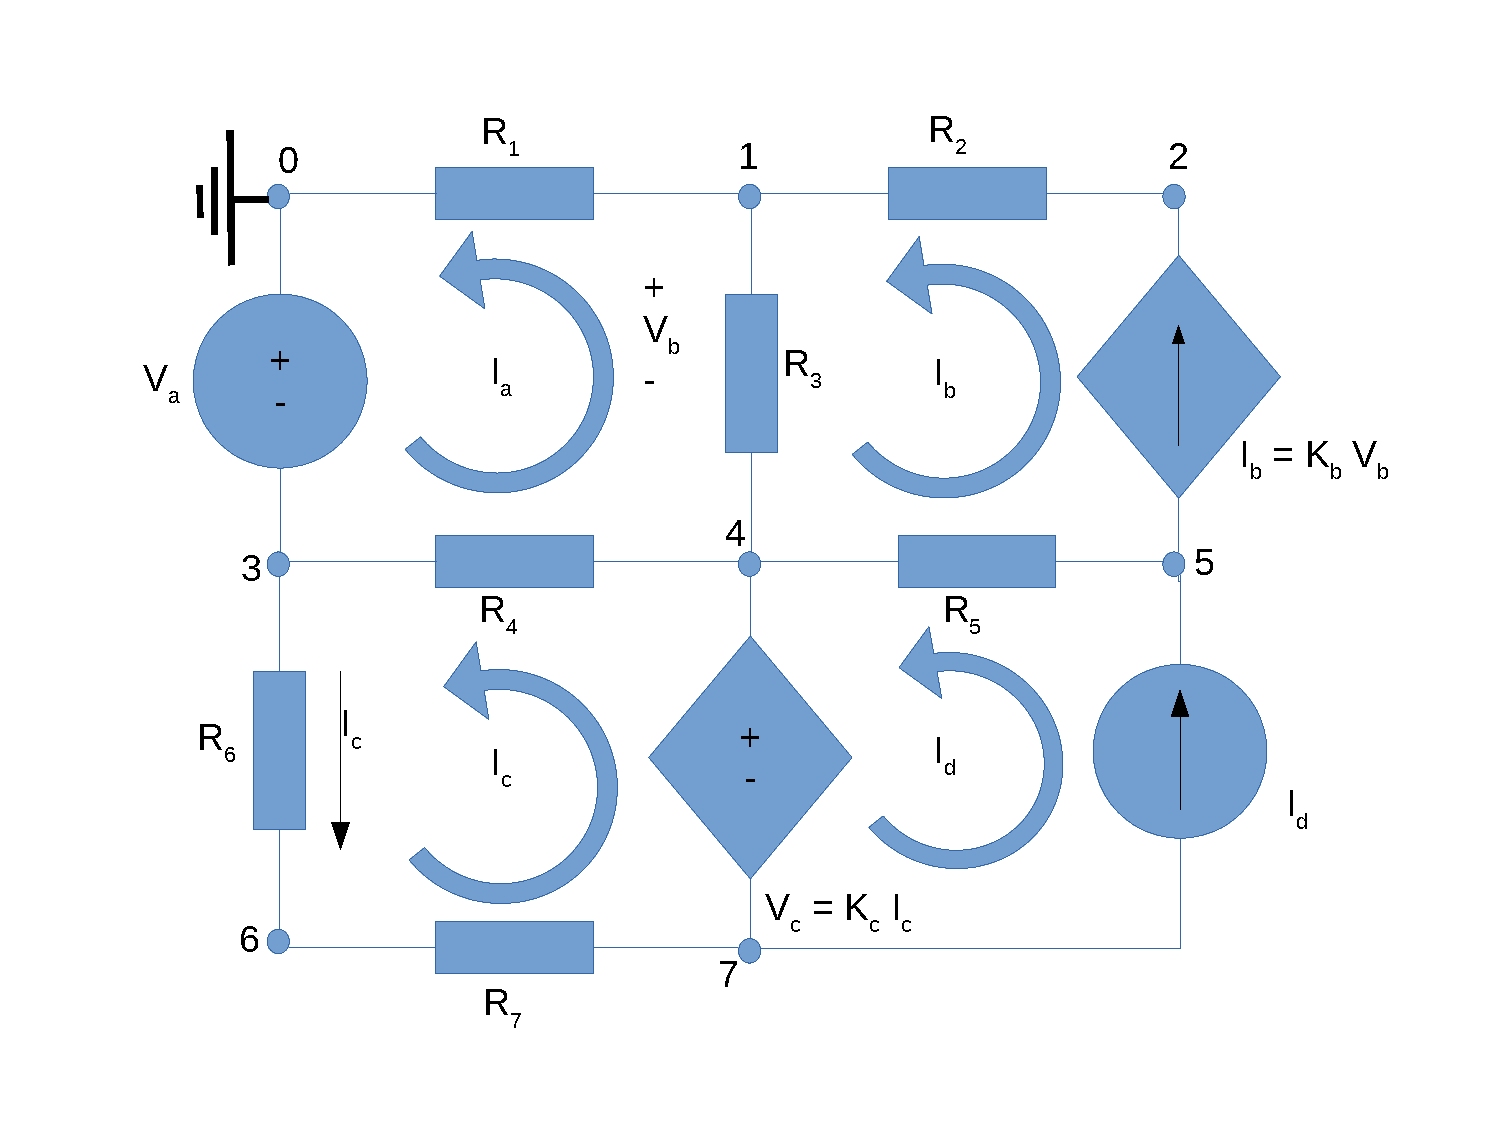
\includegraphics[width=0.4\linewidth]{t1draw.pdf}
\caption{Voltage driven serial circuit.}
\label{fig:t1draw}
\end{figure}

